\documentclass[14pt]{beamer}

\title[NST]{Neural Style Transfer}
\subtitle{NeuralArt - Stylize your Image}
\author[Team - 38]{Avishi, Vaseem Naazleen, Shivangi Tomar}
\date{June 2020}

\usetheme{Madrid}
\usepackage{graphicx}

\begin{document}

\begin{frame}
   \titlepage
\end{frame}

\begin{frame}
		\frametitle{Overview}
		Our project aims to stylize image by implenting A Neural Algorithm of Artistic Style paper by Leon A.Gatys, Alexander S.Ecker and Mathias Bethge.
        
		https://arxiv.org/pdf/1508.06576.pdf
\end{frame}

\begin{frame}
		\frametitle{What is Neural Style Transfer?}
		\setbeamertemplate{itemize items}[ball]
		\begin{itemize}
		\item Neural Style Transfer is a technique used to generate image in the style of another image.
		\item It takes a content image, a style image, and returns the content image as if it were painted using the artistic style of image.
		\end{itemize}
		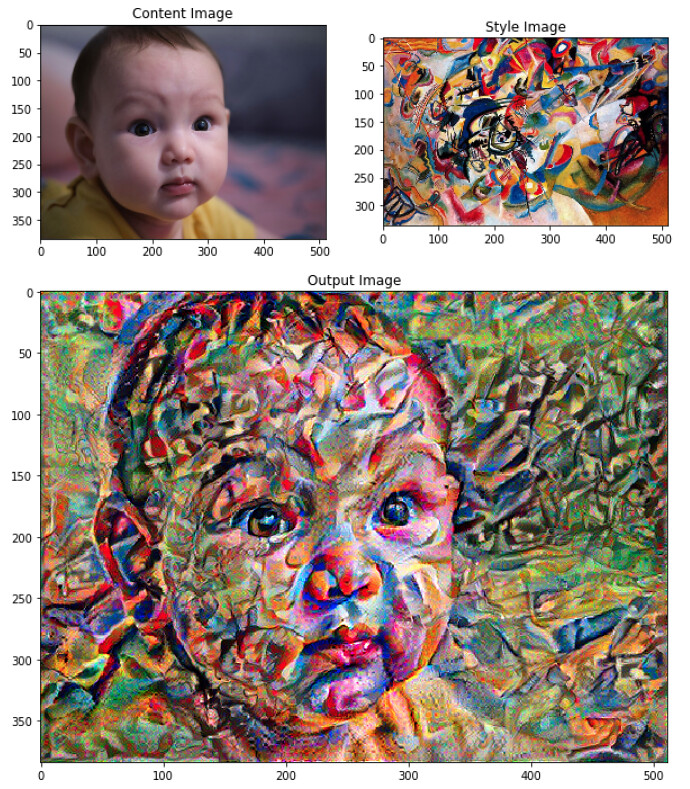
\includegraphics[width=100mm]{image.jpg}
\end{frame}

\begin{frame}
		\frametitle{Key Finding}
		The representation of content and style in the Convolutional Neral Network are seperable.
\end{frame}

\begin{frame}
		\frametitle{Modules}
		\setbeamertemplate{itemize items}[ball]
		\begin{itemize}
		\item Keras (TensorFlow backend)
		\item NumPy
		\item SciPy
		\item Flutter
		\end{itemize}
\end{frame}

\begin{frame}
		\frametitle{Status}
		\setbeamertemplate{itemize items}[ball]
		\begin{itemize}
		\item Read the research paper.
		\item Working on the code implementations.
		\end{itemize}
\end{frame}

\begin{frame}
		\frametitle{Learnings and Difficulties}
		\setbeamertemplate{itemize items}[ball]
        \begin{itemize}
		\item Learned to work with github conveniently.
		\item Learned to make presentation using Beamer.
		\item Studied about CNN.
		\end{itemize}
\end{frame}

\begin{frame}
		\frametitle{Difficulties}
		\setbeamertemplate{itemize items}[ball]
        \begin{itemize}
				\item The program is taking lot of time to output stylized image.(Working on it)
		\end{itemize}
\end{frame}

\begin{frame}
	                              	Thank You :)
\end{frame}

\end{document}
